% JUMP TO LINE 60, 73
\documentclass[preview, margin=0.6in]{standalone}
\usepackage[letterpaper,portrait,top=0.4in, left=0.6in, right=0.6in, bottom=1in]{geometry}

\usepackage{amsmath, amsfonts, amsthm, amssymb}
\usepackage{graphicx, float}
\usepackage{mathtools}
\usepackage{titlesec}
\usepackage{interval}
\usepackage{hyperref}
\usepackage{siunitx}
\usepackage{titling}
\usepackage{vwcol}
\usepackage{setspace}
\usepackage{empheq}
\usepackage{cancel}
\usepackage{esdiff}
\usepackage{multicol}
\usepackage{mdframed}
\usepackage{esdiff}
\usepackage{tikzsymbols}
\usepackage{multicol}
\usepackage{tikz}
\usepackage{varwidth}
\usepackage{pgfplots}
\pgfplotsset{compat=1.18}
\intervalconfig {
	soft open fences
}
\usepackage{tikz}
\usetikzlibrary{positioning}
\usetikzlibrary{angles,quotes}

\newcommand{\alignedintertext}[1]{%
  \noalign{%
    \vskip\belowdisplayshortskip
    \vtop{\hsize=\linewidth#1\par
    \expandafter}%
    \expandafter\prevdepth\the\prevdepth
  }%
}

\newtheorem{lemma}{Lemma}

\renewcommand{\qedsymbol}{\Smiley[1.3]}
\newcommand*{\problem}[1]{\section*{Problem #1}}
\newcommand*{\aps}{\section*{AP Corner}}
\newcommand*{\deriv}[1][x]{\ensuremath{\dfrac{\mathrm{d}}{\mathrm{d}#1}}}
\newcommand*{\floor}[1]{\ensuremath{\lfloor #1\rfloor}}
\newcommand*{\lheqzero}{\ensuremath{\underset{\text{L'H}}{\overset{\left[\frac00\right]}{=}}}}
\newcommand*{\lheqinfty}{\ensuremath{\underset{\text{L'H}}{\overset{\left[\frac{\infty}{\infty}\right]}{=}}}}

\DeclareMathOperator{\DNE}{DNE}
\DeclareMathOperator{\sgn}{sgn}

\DeclareMathOperator{\arccsc}{arccsc}
\DeclareMathOperator{\arcsec}{arcsec}
\DeclareMathOperator{\arccot}{arccot}

\setlength{\parindent}{0pt}

%opening
\title{\vspace*{-30pt}Problem Set \#17}
\author{Jayden Li}
\date{\today}

% \allowdisplaybreaks
\postdisplaypenalty=100000

\begin{document}
\setstretch{1.25}
\fontsize{12pt}{12pt}\selectfont
\setlength{\abovedisplayskip}{0pt}
\maketitle
\problem{3}
\begin{itemize}
	\item[(a)]
	\begin{minipage}[t]{0.3\linewidth}
		\begin{tikzpicture}[
			baseline=(current bounding box.north),
			ang/.style={draw, angle eccentricity=1.5,angle radius=0.6cm}
		]	
			\draw 
			(0,0) coordinate[label=below:{$A$}](A)
		 -- (3,0) coordinate[label=below:{$C$}](C) node[midway,below]{$1$}
		 -- (3,7) coordinate[label=above:{$B$}](B) node[midway,right]{$\sqrt{4x^2-1}$}
		 -- cycle node[midway,above,left]{$2x$}
			pic["$\theta$",ang]{angle=C--A--B};
		\end{tikzpicture}
	\end{minipage}
	\begin{minipage}[t]{0.33\linewidth}
		$\begin{aligned}[t]
			\cos\theta&=\frac{1}{2x} \\
			2x\cos\theta&=1 \\
			x&=\frac12 \sec\theta \\
			\mathrm{d}x&=\frac12 \sec(\theta)\tan(\theta)\,\mathrm{d}\theta \\ \\
			1&=\frac{1}{2\cos\theta}\implies\theta=\frac{\pi}{3} \\
			\frac12&=\frac{1}{2\cos\theta}\implies\theta=0
		\end{aligned}$
	\end{minipage}
	\begin{minipage}[t]{0.36\linewidth}
		$\begin{aligned}[t]
			&\int_{1/2}^{1}\frac{x^3}{\sqrt{4x^2-1}}\,\mathrm{d}x \\
			={}&\int_{0}^{\pi/3}\frac{\frac{1}{8}\sec^3(\theta)\frac12\sec(\theta)\tan(\theta)}{\sqrt{\sec^2-1}}\,\mathrm{d}\theta \\
			={}&\frac{1}{16}\int_{0}^{\pi/3}\frac{\sec^4\theta}{\cancel{\tan\theta}}\cdot\cancel{\tan(\theta})\,\mathrm{d}\theta \\
			={}&\frac{1}{16}\int_{0}^{\pi/3}\sec^2(\theta)(1+\tan^2\theta)\,\mathrm{d}\theta \\
			={}&\left[\begin{aligned}
					u&=\tan\theta \\
					\mathrm{d}u&=\sec^2\theta \,\mathrm{d}\theta
			\end{aligned}\right] \\
			\phantom{=}{}&\frac{1}{16}\int_{0}^{\sqrt3}\left(1+u^2\right)\mathrm{d}u \\
			={}&\frac{1}{16}\left[u+\frac{u^3}{3}\right]_{0}^{\sqrt3}
			=\boxed{\frac{\sqrt{3}}{8}}
		\end{aligned}$
	\end{minipage}
\end{itemize}

\problem{4}
\begin{minipage}[t]{0.27\linewidth}
	\begin{tikzpicture}[
		baseline=(current bounding box.north),
		ang/.style={draw, angle eccentricity=1.5,angle radius=0.6cm}
	]	
		\draw 
		(0,0) coordinate[label=below:{$A$}](A)
	 -- (2.5,0) coordinate[label=below:{$C$}](C) node[midway,below]{$1$}
	 -- (2.5,5) coordinate[label=above:{$B$}](B) node[midway,right]{$\sqrt{x^2-1}$}
	 -- cycle node[midway,above,left]{$x$}
		pic["$\theta$",ang]{angle=C--A--B};
	\end{tikzpicture}
\end{minipage}
\begin{minipage}[t]{0.3\linewidth}
	$\begin{aligned}[t]
		\cos\theta&=\frac{1}{x} \\
		x&=\sec\theta \\
		\mathrm{d}x&=\sec(\theta)\tan(\theta)\,\mathrm{d}\theta \\ \\
		1&=\sec\theta \\
		\implies \theta&=\arcsec1=0 \\
		7&=\sec\theta \\
		\implies \theta&=\arcsec7 \\ \\
		\tan\theta&=\sqrt{x^2-1}
	\end{aligned}$
\end{minipage}
\begin{minipage}[t]{0.37\linewidth}
	$\begin{aligned}[t]
		&\int_{1}^{7}\frac{\sqrt{x^2-1}}{x}\,\mathrm{d}x \\
		={}&\int_{0}^{\arcsec7} \frac{\sqrt{\sec^2\theta-1}\cdot\sec\theta\tan\theta}{\sec\theta}\,\mathrm{d}\theta \\
		={}&\int_{0}^{\arcsec7} \tan^2\theta\,\mathrm{d}\theta
		=\left[\tan\theta-\theta\right]_{0}^{\arcsec7} \\
		={}&\left.\sqrt{x^2-1}\right|_{1}^{7}-\left.\theta\right|_{0}^{\arcsec7}
		=\sqrt{48}-\arcsec7 \\
		={}&4\sqrt3-\arcsec7
	\end{aligned}$

	$\begin{aligned}[t]
		&\text{Average}
		=\frac{1}{7-1}\int_{1}^{7}\frac{\sqrt{x^2-1}}{x}\,\mathrm{d}x \\
		={}&\frac16\left(4\sqrt3-\arcsec7\right)
		=\boxed{\frac{2 \sqrt{3}}{3}-\frac{\arcsec7}{6}}
	\end{aligned}$
\end{minipage}

\problem{5}
\begin{itemize}
	\item[(a)]
	\begin{minipage}[t]{0.19\linewidth}
		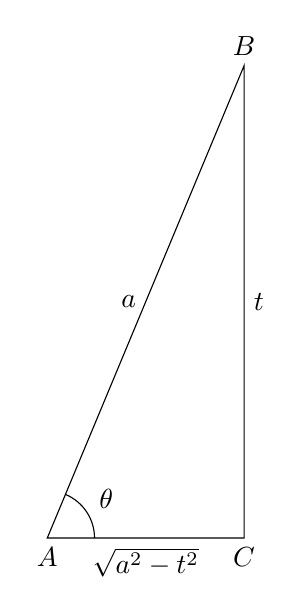
\begin{tikzpicture}[
			baseline=(current bounding box.north),
			ang/.style={draw, angle eccentricity=1.5,angle radius=0.6cm}
		]	
			\draw 
			(0,0) coordinate[label=below:{$A$}](A)
		 -- (2.5,0) coordinate[label=below:{$C$}](C) node[midway,below]{$\sqrt{a^2-t^2}$}
		 -- (2.5,6) coordinate[label=above:{$B$}](B) node[midway,right]{$t$}
		 -- cycle node[midway,above,left]{$a$}
			pic["$\theta$",ang]{angle=C--A--B};
		\end{tikzpicture}
	\end{minipage}
	\begin{minipage}[t]{0.21\linewidth}
		$\begin{aligned}[t]
			\sin\theta&=\frac{t}{a} \\
			t&=a\sin\theta \\
			\mathrm{d}t&=a\cos\theta \,\mathrm{d}\theta \\ \\
			0&=a\sin\theta \\
			\implies\theta&=0 \\ \\
			x&=a\sin\theta \\
			\implies\theta&=\arcsin\frac{x}{a}
		\end{aligned}$
	\end{minipage}
	\begin{minipage}[t]{0.59\linewidth}
		$\begin{aligned}[t]
			&\int_{0}^{x}\sqrt{a^2-t^2}\,\mathrm{d}t
			=\int_{0}^{\arcsin\frac xa}\sqrt{a^2-a^2\sin^2\theta}\cdot a\cos\theta\,\mathrm{d}\theta \\
			={}&a^2\int_{0}^{\arcsin\frac xa}\cos^2\theta\,\mathrm{d}\theta
			=\frac{a^2}{2}\int_{0}^{\arcsin\frac xa}(1+\cos2\theta)\,\mathrm{d}\theta \\
			={}&\frac{a^2}{2}\left[\theta+\frac{ \sin2\theta}2\right]_{0}^{\arcsin\frac xa}
			=\frac{a^2}{2}\left[\arcsin\frac xa+\frac{\sin\left(2\arcsin\frac xa\right)}2\right] \\
			={}&\frac{a^2}{2}\left[\arcsin\left(\frac xa\right)+\frac{2\sin\left(\arcsin\frac xa\right)\cos\left(\arcsin\frac xa\right)}{2}\right] \\
			={}&\frac{a^2}{2}\left[\arcsin\left(\frac xa\right)+\frac xa\cdot \frac{\sqrt{a^2-x^2}}{a}\right] \\
			={}&\boxed{\frac12a^2\arcsin\left(\frac xa\right)+\frac12x \sqrt{a^2-x^2}}
		\end{aligned}$
	\end{minipage}

	\item[(b)] The area bound by a circle, the $y$-axis, and some line between the $y$-axis and the intersection of the circle with the $x$-axis equals $\displaystyle\frac12a^2\arcsin\left(\frac xa\right)+\frac12x \sqrt{a^2-x^2}$ if $x$ is the $x$-value of the line.
\end{itemize}

\end{document}
